\newSec{Regelkreis}{2}

Im Allgemeinen grenzen sich die Konzepte \textit{steuern} und \textit{regeln} durch die Eigenschaft der Rückkopplung des Systems ab. Gesteuerte Systeme wirken lediglich auf Aktoren, wobei geregelte Systeme die Abweichung des \textit{Ist}-Zustandes vom \textit{Soll}-Zustand ermitteln und eine geeignete Veränderung erzielen sollen.\comp{IEC60050-351}




\begin{figure}[ht!]
\vspace{0.25cm}
\begin{center}
\fbox{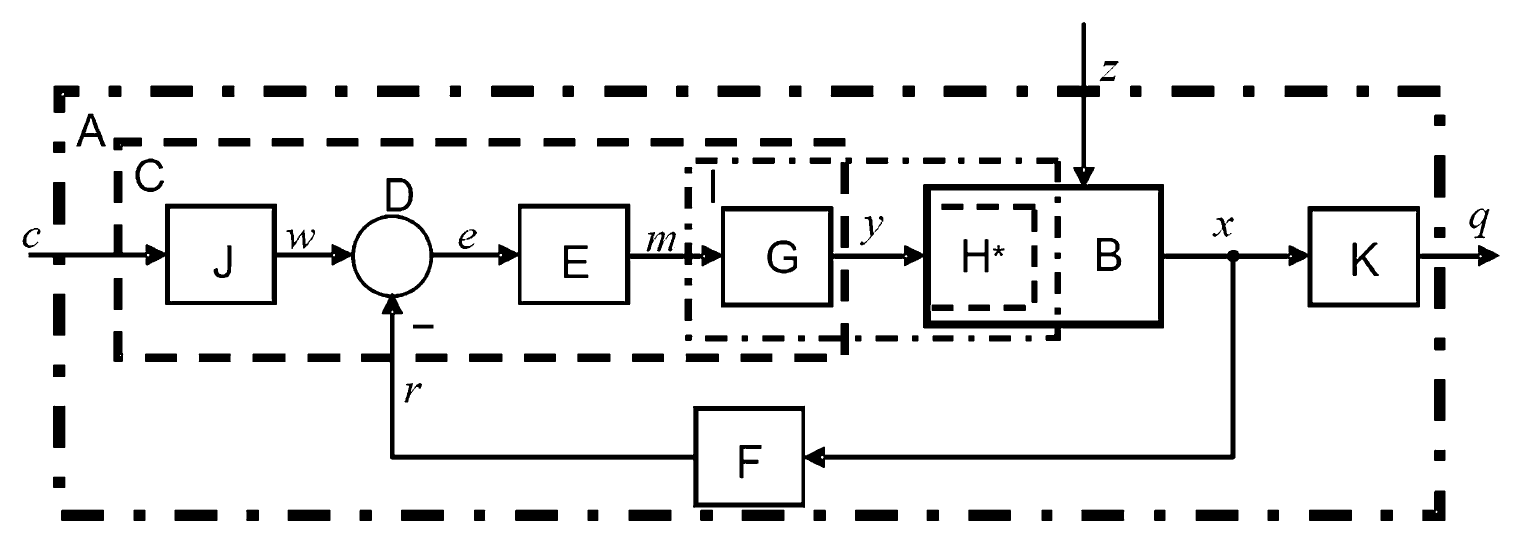
\includegraphics[width=15cm]{Pictures/Control Schema.png}}

\begin{tabular}{ll|ll}
	A  & Regelungssystem       & K & Bildung der Aufgabengröße \\
	B  & Regelstrecke          & c & Zielgröße                 \\
	C  & Regeleinrichtung      & w & Führungsgröße             \\
	D  & Vergleichsglied       & e & Regeldifferenz            \\
	E  & Regelglied            & m & Reglerausgangsgröße       \\
	F  & Messglied             & y & Stellgröße                \\
	G  & Steller               & z & Störgröße                 \\
	H* & Stellglied            & x & Regelgröße                \\
	I  & Stelleinrichtung      & q & Aufgabengröße             \\
	J  & Führungsgrößenbildner & r & Rückführgröße            
\end{tabular}
\caption{Allgeimeines Schema eines Regelkreises nach orm \textit{IEC60050-351} \cite{IEC60050-351}}
\label{fig:Contr}
\end{center}
\vspace{0.25cm}
\end{figure}






